\chapter{Concept and Design}
\label{cha:conceptanddesign}

In this section the concept and design of the artifact will be explained in greater detail.

\section{Requirements}

The following nonfunctional requirements address the specified challenges of decentralized service registries as described in the proposal. 
Furthermore, as the proposed solution make use of DLT, requirements for the design of blockchain-based applications have to be taken into account as well. These requirements will guide the concept and design phase of the artefact. 

\begin{enumerate}
    \item \textbf{Distributed Control and Management}
    The service registry is governed and orchestrated by the community and not a single central authority. 
  
    \item \textbf{Data ownership by User}
    The user is in control of his own data and can share specified user data on his own will. 
  
    \item \textbf{Sybil-attack resistancy}
    The identity of participating users are real-world identities. This is especially important in order to prevent sybil attacks. 
  
    \item \textbf{Service Quality}
    There is a way for the users to verify the quality of a service. 
  
    \item \textbf{Authenticity of provided Service Information}
    There is a way for the users to verify the authenticity of provide service information. 
  
    \item \textbf{Low Transaction costs}
    Blockchain technology favors data reliability and integrity over storage space. Storing service description data on the blockchain is expensive. 
    The costs of using the service registry should be low. 
  
  \end{enumerate}

These nonfunctional requirements will guide design decisions of the architecture of Dmarket. 

\section{Use Cases}

The following presented use cases will demonstrate the benefits of the prototype in contrast to the shortcomings of current solutions described in the proposal. 

\subsection{USE CASE 1: Signing Up}
Open decentralized systems have the problem of identity authenticity. Every user can sign up, introducing the possibility for sybil attacks. DMarket provides DID based authentication based on verified claims, thus preventing Sybil attacks and fake identities. 

\subsection{USE CASE 2: Browsing Services}
Bob sees service description of A. But he cannot verify authorship of A, nor can he verify the time stamp of listed service descriptions. Dmarket provides tamperproof and authentic lookup of services. 

\subsection{USE CASE 3: Access Control}
User A creates an Organization A and creates within that organization app A and invites user B as a member. User B now wants to edit app A.
Restricting access to app A is a challenging task in decentralized environments, since there is no central point to handle access control. DMarket uses blockchain based Identity Management through Smart Contracts, to ensure secure decentralized access control. 

\subsection{USE CASE 4: Service Rating}
P2P Reputation systems act as trust systems in order to establish trustworthiness of content. However the most prevalent challenge to those are sybil attacks, and therefore questionable trust in review reliability. Dmarket ensures trustworthy reviews by review rating calculation based on verified users. 

\section{Architecture} 
% In diesem Kapitel soll dem Leser dargelegt werden, wie mein System aufgebaut ist und warum es so aufgebaut ist. Dazu werden zunächst Real World Examples analysiert und Paper rangezogen und deren Anwendungen hinsichtlich der Anforderungen analysiert. Ausgehend davon werden Entscheidungen zum Design des Prototypen getroffen. 

In this chapter, the architecture of the system will be explained and why certain architectural choices has been made. First, a literature review regarding best practices is being conducted and based on that,  
design decisions to the relevant components of Dmarket will be explained in greater detail. 

% What do I have to pay attention to when designing a blockchain based application

Generally, the overall architecture of a blockchain-based application consists of the following components as depicted in the following figure. 

\begin{figure}[htbp]
    \centerline{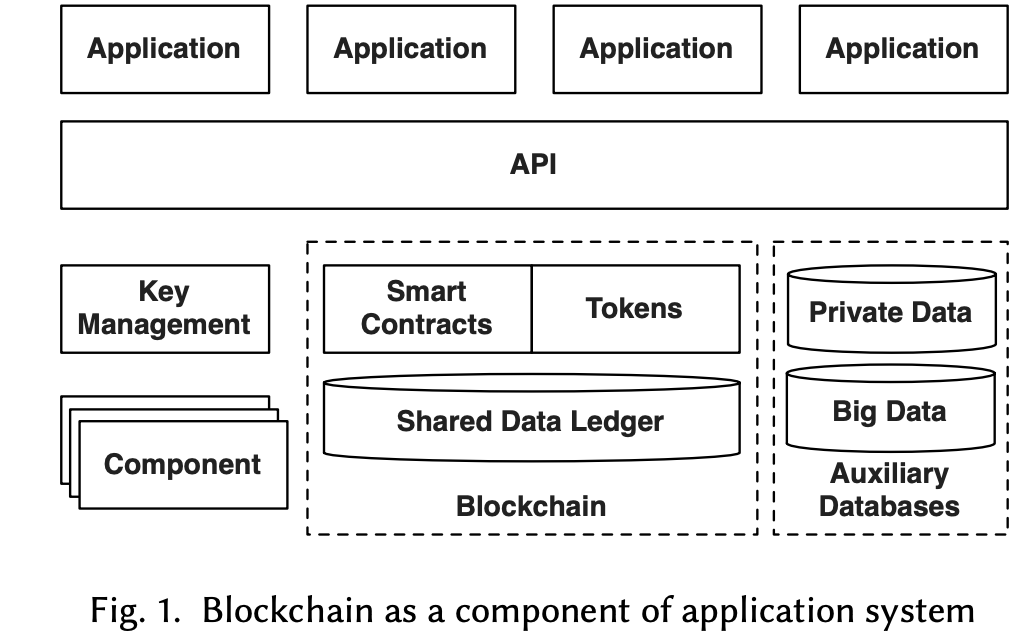
\includegraphics[width=0.9\textwidth]{images/architecture.png}}
    \caption{blockchain-based software application \label{fig:techstack} \cite{xuPatternCollectionBlockchainbased2018}}
\end{figure}

Due to its unique traits blockchain acts as a persistent, immutable and distributed data storage component in the overall architecture. As they are based on public-private key cryptography, there has to be a component, which is responsible for key management. Data which is too big, is stored in auxiliary databases and references are being stored on the blockchain. On top of the data storage layer, there is an API layer as seen in conventional applications. For the design of the prototype, a design process specified by Xu et al. has been used as an orientation. 

\textbf{Public or private ledger?}
Private Chains are not fully decentralized, whereas public chains have several challenges but can be tackled with. For a decentralized marketplace, it has to be assessed which property is more important. As described in the problem statement, a fully decentralized marketplace with no central authority and single point of failure has been defined as a requirement. Therefore fundamental properties will be the leading deciding factor.

The artefact should allow for anonymous payments and users also should be able to browse the marketplace without registering. 

Therefore a public and permission-less blockchain has been chosen. 

\textbf{data structure}
scalability, transaction costs, transaction time and network traffic and reliability has to be assessed. Blockchain offers the most trust which is needed in the application, thats why a blockchain has been decided upon. 

\textbf{on-chain or off-chain storage and computation?} 
In order to store value on the blockchain, each transaction is attached with a fee and therefore makes on-chain storage of data quite expensive.
The common way to circumvent this, is to store raw data off-chain and then to store the reference hash of the raw data on the blockchain since the amount of computational power and data storage space in the blockchain is limited. Off-chain data storage can be a private cloud/storage or public storage service provided by a third-party.  

 

%Author Xiui et al. proposes 4 common architectural patterns for integrating blockchain as part of the overall software system. Depending on the use case and requirements of a decentralized application, each pattern will have its advantages and disadvantages. Overall goal of applying those patterns is to decrease the impact of blockchain limitations and enhance its unique characteristics. According to the author, there do exist 4 different pattern types, which consist of external world patterns, contractual patterns, security pattern and data management pattern as can be seen in figure. 
% \cite[p. 52]{xuPatternCollectionBlockchainbased2018}


% \subsubsection {Motivation Blockchain Usage}
%Blockchain offer great capabilities for decentralized access control and registry services achieved through decentralized consensus and tamperproof storage of data and therefore will be used as backend of the artifact. 

\subsection{System Context}

In the domain of decentralized application marketplaces, there are the following actors: 

\subsubsection{Consumers}
The consumer party consists of one or more people, such as a private individual or employees of a company. They buy certain services, which are offered by service providers. 

\subsubsection{Service Provider}
Service provider can also be private individuals or companies. They sell their digital services to the consumer/costumer. 

\subsubsection{Identity Validators}
Independent organizations, who are allowed to issue verifiable identity claims. 

\subsubsection{App Validators}
independent organizations, who are allowed to issue verifiable claims about app quality. 

\subsection{Overview}
The blockchain-based application is implemented on top of the decentralized infrastructure mentioned in the introduction, called Blade. The following figure provides an overview of the components which are briefly described. 

\begin{figure}[htbp]
    \centerline{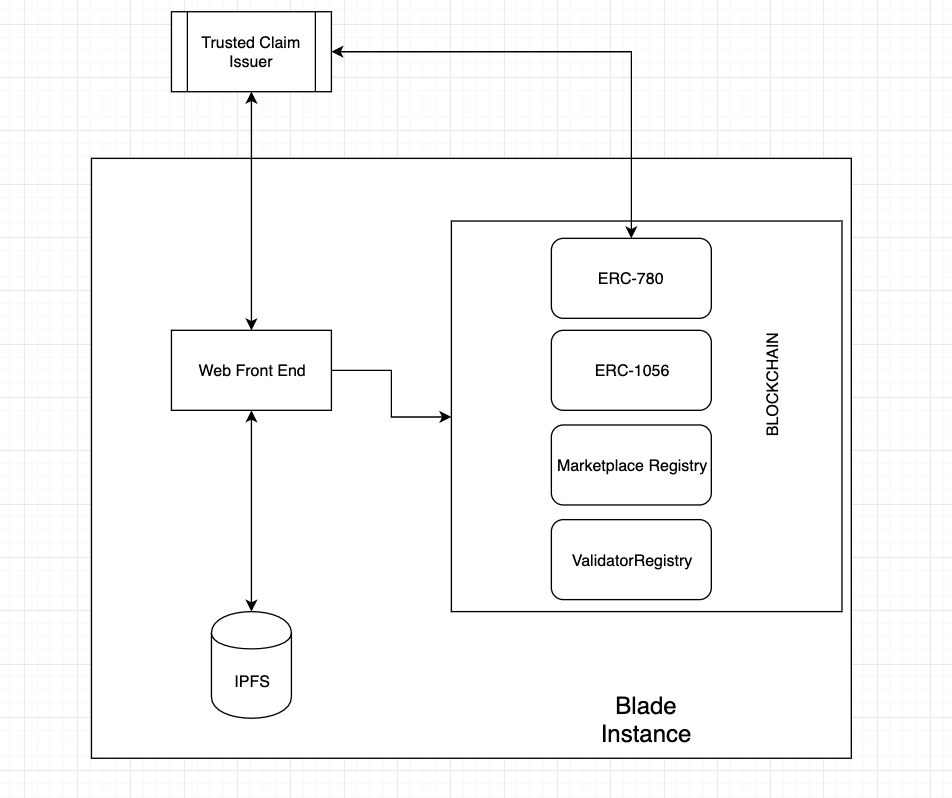
\includegraphics[width=0.9\textwidth]{figures/overview.png}}
    \caption{Architecture overview \label{fig:techstack}}
\end{figure}

\begin{enumerate}
    \item \textbf{Blade instance:}
    a machine having a blade instance installed providing the user with different interfaces in order to use the decentralized infrastructure including identity management and a marketplace interface. 
  
    \item \textbf{web frontend:} The web front end is the GUI user interface which allows the users to use the functionalities of the decentralized marketplace. 
  
    \item \textbf{distributed data storage IPFS:} The client can store its marketplace-related claims publicly available to its marketplace users. The storage is distributed and therefore accessible by other users even when the client is offline.  
  
    \item \textbf{blockchain component} This component contains several smart contracts dealing with data storage and providing access control functionality as well as decentralized identity management and data verification services. 
    
    \item \textbf{Registry server} The registry server fetches the blockchain log events and stores entity data on a local server. This increases look up time and query time for marketplace related data. 
    The server queries the DIDAttributeChanged of all Identities 
  
    \item \textbf{trusted claim issuers} These are trusted identity and app validators who issue claims for apps registered in the marketplace. people who upload app will need to get their apps certified by these independent validators. Validators will get a token and if the marketplace grows the token grows in value. Other users can now also buy apps with that token, so there is an economy surrounding the whole marketplace. 
  
\end{enumerate}

\subsection{API} 

The most important REST endpoints of the Registry server will be described in the following. 

Entity related data is stored tamperproof on the blockchain and IPFS storage. While data reliability and integrity is being enhanced greatly by the use of blockchain, data queriablity is very slow. In order to enhance this performance, a registry server will synchronize the data and store it in a local database such as e.g. mongodb, which offers sophisticated and fast query methods. 

\textbf{apps}

\begin{figure}[htbp]
    \centerline{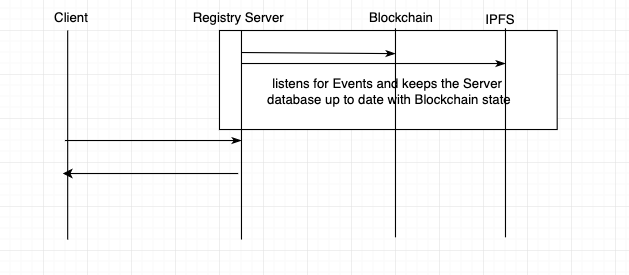
\includegraphics[width=0.9\textwidth]{figures/RegistryServer.png}}
    \caption{Fetching data \label{fig:registryServer}}
\end{figure}

\begin{table}[hbt!]
    \centering
    \caption{App}
    \begin{tabular}{llll}
    Method & Path      & Description         &   \\
    GET    & /apps     & get all Apps~       &   \\
    GET    & /apps/:id & get a specific app~ &   \\
           &           &                     &  
    \end{tabular}
\end{table}

\textbf{organizations} 

\textbf{apis}

\subsubsection{DIDResolver}

The DIDResolver builds upon the Ethr-DID-Resolver developed by uport, which enables ethereum addresses to be managed as decentralized identifiers compliant to the W3C specification. Every identity on the marketplace is represented through such a DID and its respective JSON document. The server uses this DID Resolver to resolve the decentralized IDs to their records. The DID Document for an app created in the marketplace looks like this: 

\begin{lstlisting}[caption={AppVersion}, language=Solidity, label=lst:appVersionFormat, numbers=none]
    {
      "@context": "https://w3id.org/did/v1",
      "id": "did:uport:2nQtiQG6Cgm1GYTBaaKAgr76uY7iSexUkqX",
      "publicKey": [{
        "id": "did:dmarket:2nQtiQG6Cgm1GYTBaaKAgr76uY7iSexUkqX#keys-1",
        "type": "Secp256k1VerificationKey2018",
        "owner": "did:dmarket:2nQtiQG6Cgm1GYTBaaKAgr76uY7iSexUkqX",
        "publicKeyHex": "04613bb3a4874d27032618f020614c21cbe4c4e4781687525f6674089f9bd3d6c7f6eb13569053d31715a3ba32e0b791b97922af6387f087d6b5548c06944ab062"
      }],
      "authentication": [{
        "type": "Secp256k1SignatureAuthentication2018",
        "publicKey": "did:dmarket:2nQtiQG6Cgm1GYTBaaKAgr76uY7iSexUkqX#keys-1"
      }],
      "dMarket": {
        "@context":"http://schema.org",
        "@type":"AppVersion",
        "app":"did:dmarket:3234234234234234234234",
        "version":"2", 
        "description":"Uport Attestations",
        "image":{"@type":"ImageObject","name":"avatar","contentUrl":"/ipfs/QmSCnmXC91Arz2gj934Ce4DeR7d9fULWRepjzGMX6SSazB"}
        "binaryLink": {"@type":"URLObject"},
        "supportedAPI":[]
      }
    }
\end{lstlisting}


\section{Identity Management}

Each service, organization or user is represented as an identity. Identities are represented by their Ethereum addresses. With the ERC-1056, those addresses are fully compliant to the WC3 DID Specification, thus each identity can be resolved to their respective DID document. 
Following assumptions regarding identity claim issuers have been made: there are trusted identity issuers existent, who issue verifiable identity claims to their subjects. Also they register a hash of that claim on the claim registry ERC780, mapping it to the specific subject of claim. 

\subsection{Registration of users}

The following figure provides an overview about the request flow made, when registering a user for the marketplace. 

\begin{figure}[htbp]
    \centerline{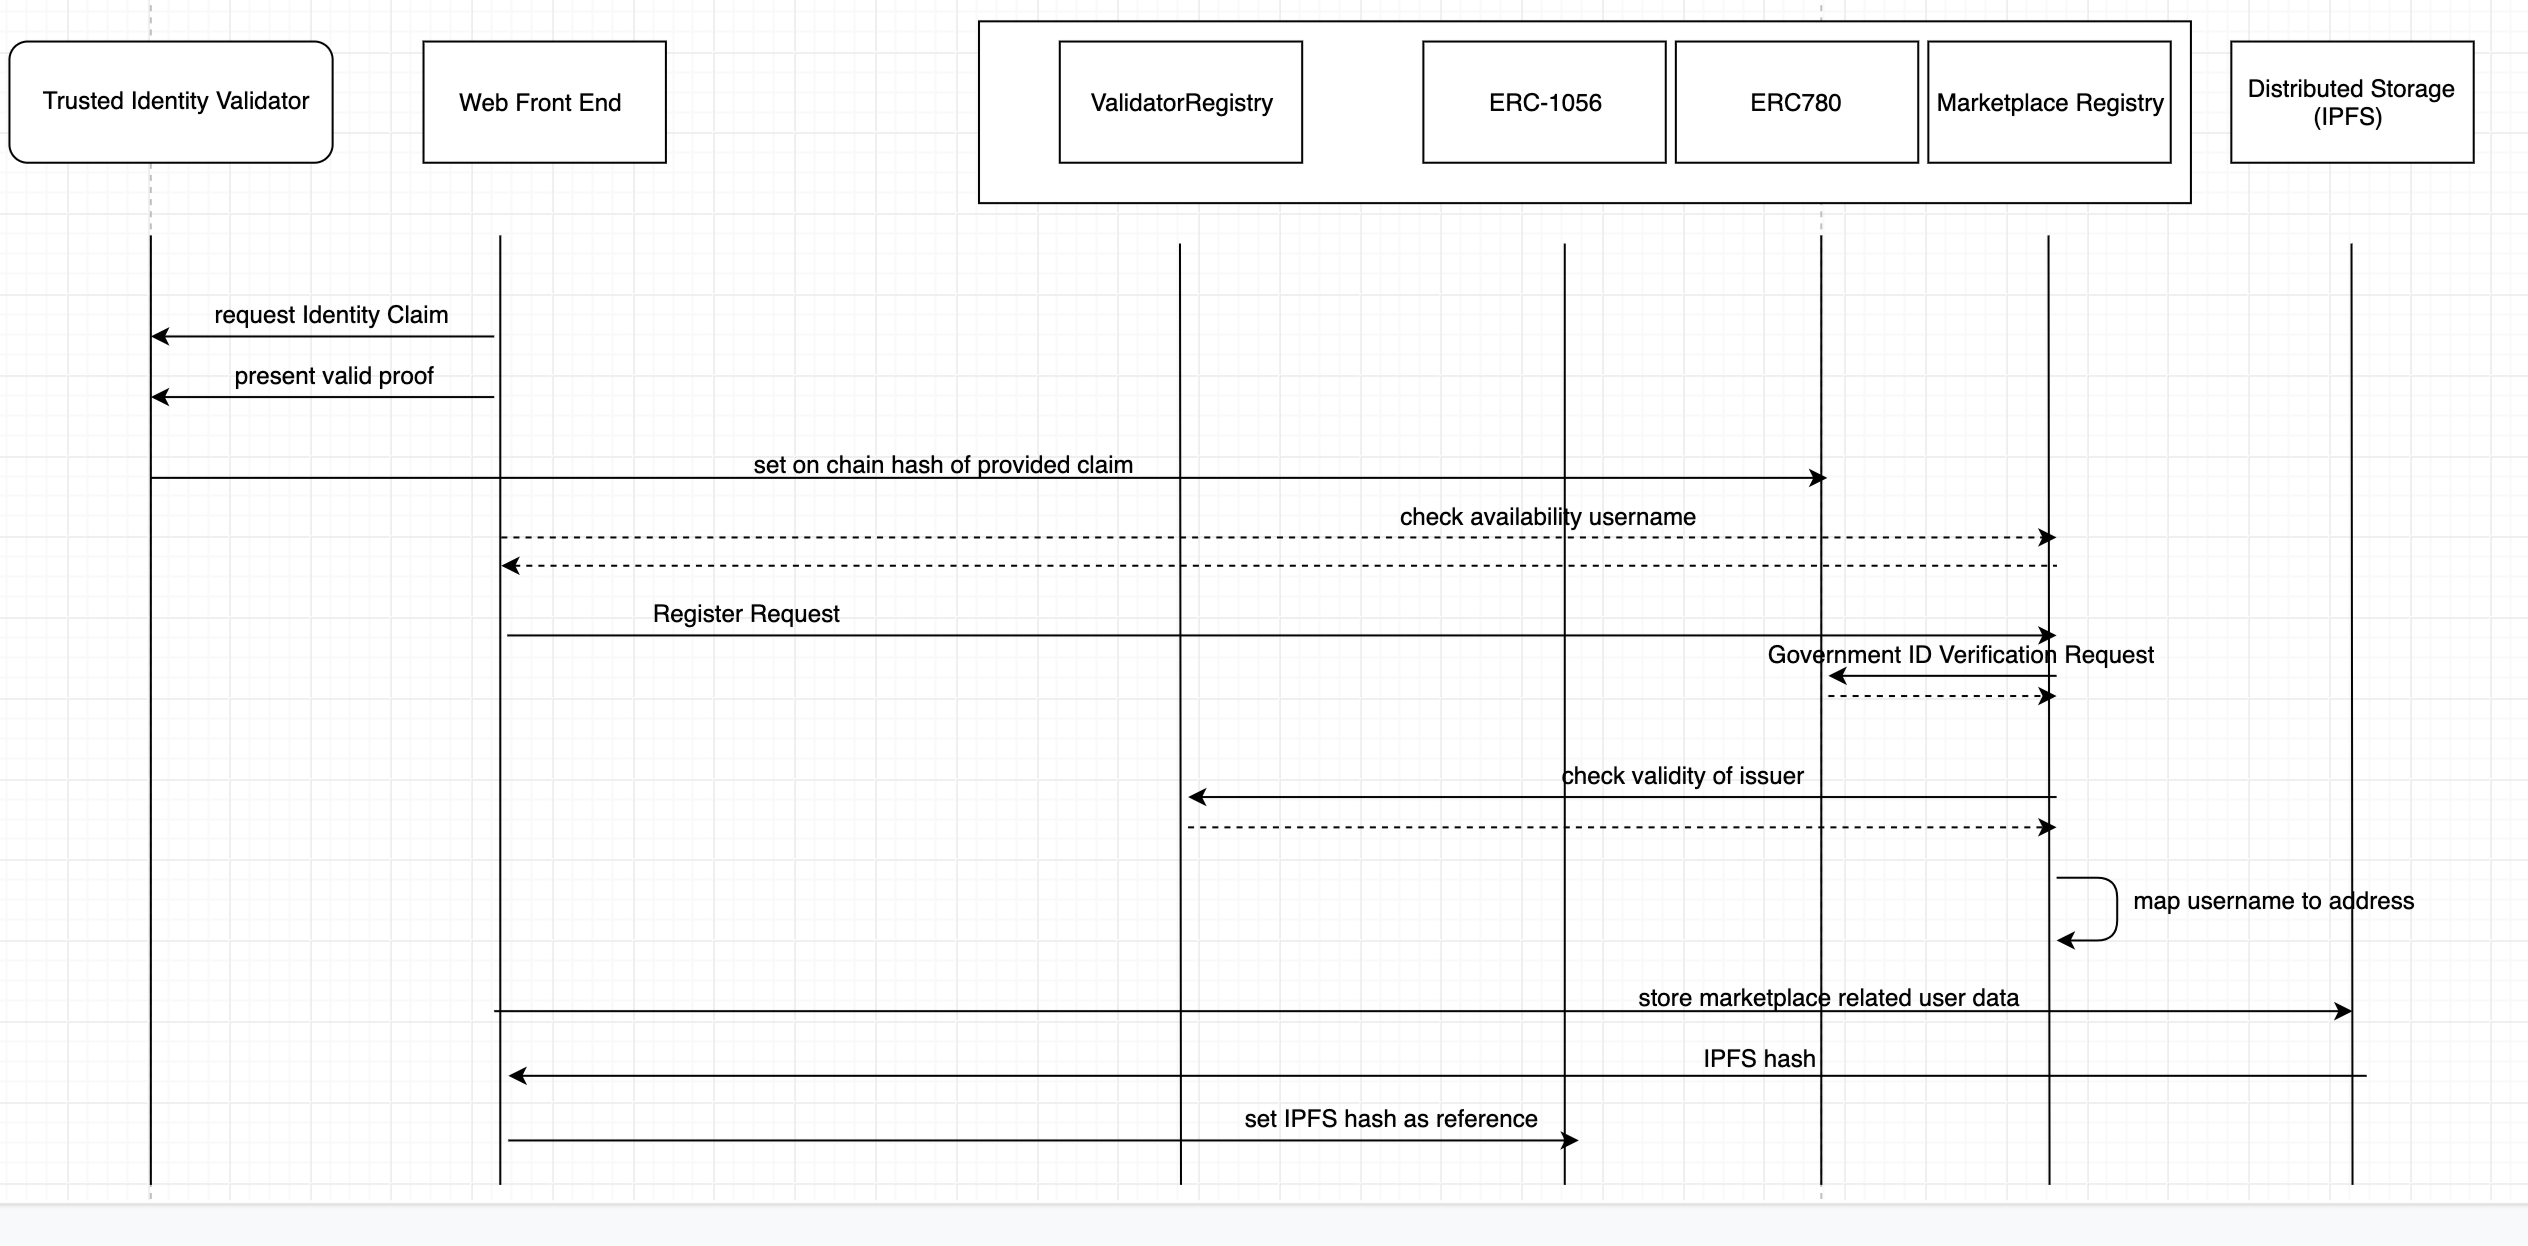
\includegraphics[width=0.9\textwidth]{figures/userRegistration.png}}
    \caption{Registration process \label{fig:registration}}
\end{figure}

Before registering on the marketplace, the user will be prompted to verify his identity at one of the accepted government ID validators. In this implementation, a stub validator will be implemented and we will assume that this entity is trustworthy. Once verified, the claim will be registered onchain. 

Now when registering a username, the marketplace registry will check for the government ID claim at the on-chain registry ERC-780 and if verification is successful, he will be able to register his username.

\subsection{Registration of Apps, Apis, Organizations}

Once a username is registered, he can register apps, api and organizations. Those will be called "entity" in the following. The registration consists of two steps: 
First, for each entity an Ethereum account will be created.
This public key will then be registered in the marketplace registry, which essentially acts as a name registry assigning human-friendly names on a first come, first served basis. 
When creating entities, the ownership over their DID documents will be transferred to the user, who created them. The registration of apps requires a marketplace specific claim verification schema, which has been showed in the data structures section. The marketplace registry has therefore a verification function, which will check wether the entity to be uploaded in IPFS conforms to that schema.

\section{Content Model}

Every User, App or Api, or Organization represents an identity and is being referenced by a unique decentralized identifier. This identifier follows the specification of a DID Document. Using decentralized identity fullfils the requirement of self souvereign data ownership. Each identity is being managed by its respective owner, and all data attached to that identity therefore belongs to them. 

% Every created entity is owned by its author. So in the normal case, the author is the same as the owner. But in case, that a user is creating a entity in the context of his organization, owner will be the organization. In either case, these roles are specified in the blockchain through cryptographic key management.  

\subsection{Related Work}

%{Decentralized Identifier} 

%{DID URL}

\subsection{Content Model}

This following content model conforms to the general DID specification. This data is being retrieved from the blockchain and will be presented as such by the DID resolver method. 

% THIS FUCKS UP THE FORMATTING. 
\begin{lstlisting}[caption={Example app content object}, language=Solidity, label=lst:content_model, numbers=none]
{
    "@context": "https://www.w3.org/ns/did/v1",
    "id": "did:example:123456789abcdefghi",
    "authentication": [{
        "id": "did:example:123456789abcdefghi#keys-1",
        "type": "RsaVerificationKey2018",
        "controller": "did:example:123456789abcdefghi",
        "publicKeyPem": "-----BEGIN PUBLIC KEY...END PUBLIC KEY-----"
    }],
    'dmarket': {
        '@context': 'http://schema.org',
        '@type': 'App',
        'name': 'Tawki',
        'owner': 'Microsoft',
        'author': "did:ethr:john"
        'description': 'Tawki is a decentralized chatting app making you feel very happy.',
        'image': {'@type': 'ImageObject', 'name': 'avatar', 'contentUrl': '/ipfs/QmSCnmXC91Arz2gj934Ce4DeR7d9fULWRepjzGMX6SSazB'},
        'versions': [{id:"...", type: "version", rating: "1.5"}, {id:"...", type: "version", rating: "2.5"}
    },
    "service": [{
        "id":"did:example:123456789abcdefghi#vcs",
        "type": "VerifiableCredentialService",
        "serviceEndpoint": "https://example.com/vc/"
    }]
}   
\end{lstlisting}


\subsection{Access Control Model}
% What is the goal of this model? User should be able to create organizations and assign control rights to added users. 

The goal of this model is to specify how access control can be handled with blockchain technology. If every organization or user could specify its own rules it actually would be optimal. Right now, role-based access control is being implemented. 

There is the possibility for app developers to create organizations and inviting multiple developers the organization. Therefore the attribute author specifies the person who created the entitiy (e.g. app or api), whereas owner specifies the ownership about the entity. For example, if Bob create an organization and invites Alices to the organization, he can choose to assign her one of those roles: Admin or Member. If Alice now creates an app within that organization, the app is owned by that organization but has been authored by Alice. If alice would leave the organization, then she would loose rights to edit this entity. 

\subsubsection{Roles} 
Those following roles do exist for the user. A user can be part of an organization and therefore gets a role assigned, if he joins an organization. Besides that, every user who creates an entity has the role of an author. Being the author usually means automatically being the owner as well, but not if he is part of an organization. 

\begin{enumerate}
    \item \textbf{Author:} The authorship authorizes the user to create, update or delete an entity.

    \item \textbf{Owner:} Being owner of an entity authorizes him/her to grant access to ressources of the marketplace. 

Within organizations: 

    \item \textbf{Admin:} The admin role authorizes the user to edit all entities within that organization. The admin has also the right to invite other users to the organization. 
    
    \item \textbf{Member:} being a member means to be able to create and edit their own entities within that organization. But they are not allowed to invite other members or edit the other entities besides their own. 
\end{enumerate}

\subsection{Service discovery}

% Registry Server Explanation

The DID Documents of registered entities will be resolved by a DID resolver. 
Since a public blockchain is being used, each transaction recorded is visible to everyone. The EIP712 proposal makes it possible to sign structured data to make verifiable off chain claims possible. For public apps or apis, the reference is stored on-chain as a DID attribute of their respective DID documents. This makes fetching the data more accessible. If the user would want to keep this data claims private, they could provide an endpoint from which other users could request this data. Another possibility would be to encrypt this data object with a secret via symmetric encryption and other users could request that secret in order to decrypt it. 



\subsection{Trust Mechanism}

\subsubsection{Sybil Attacks} 


\subsubsection{Service Quality}

This whole prototype is being designed with the idea of integrating decentralized identity in order to create trust while preserving the privacy of its users. In order to prevent sybil attacks and create trust in identity of app providers, users have to acquire a verifiable claim from the marketplace. The IdentityValidatorRegistry smart contract acts as a verifying instance. It will hold a list of trusted government ID validators and users will have to get their identity verified by these entities first. The marketplace will then authenticate user identity based on those claims, which will enable the users to interact on the service registry. 

Users who use that service registry can therefore be sure, that all provided apps are from real-world identities, without knowing any private information about those identities. 
Furthermore, to enhance trust in quality of apps, app validators could issue verifiable claims about the quality of those apps, too. 



\subsection{Verifiable Claims}
The DID Document is fetched  from the authenticator. It is fetched from a Verifiable Data Registry! The  Verifiable Data Registry holds all Deentralized Identities and their Keys. 

The authenticator/ verifier can verify all signed data by that registry. 

Because the registry holds the data schema for that OFF chain data, and the identifier/key used in conjunction with the issuer of the data is registered. One can verify that this data is conforming to that schema and has been signed by that authority. 

The schema is important because it defines the structure of the claim, and also an explanation of the claim, what validators can expect from it. 


Now the problem is my marketplace is a smart contract. It does not have authentication keys. It doesn'T sign messages with a signature. 

A way to solve this is with an onchain Claim. 

We don't resolve the DID document of marketplace and check for the signature, but we ask ERC780 for validation. 

Now the cool thing about verifiable Claims is, that the claim itself is a readable JSON in the structure already. It can be nested and complex as fuck, it doesnt matter since only the signature of it matters. And because the signature is deeply coupled with the content, once I use that signature and that hash and it returns me the public key , i Know it has not been altered and I know yeah, that claim is valid. The subject know just has to proof that he is the subject and then it is alright. 

Now because the smart contract cannot sign that verifiable Claim, I will just let the subject sign that shit! 

This will generate me a signature. 

Issuer  : Marketplace 
Subject: Subject Address
Data : Hash  / Claim ID, Claim Key  

Verification 

Take Data verify its schema -> Check. 
Signature is not needed, because the client will have to check that issuer in the claim indeed is the issuer address set in ERC780. 

Now hash that claim with 